\documentclass{article}
\usepackage[utf8]{inputenc}
\usepackage{amsmath, amssymb, amsthm}
\usepackage[margin=1in]{geometry}
\usepackage{graphicx}  % For including images
\usepackage{listings}  % For including code
\usepackage{xcolor}  % For code highlighting
\usepackage{subcaption}  % For subfigures
\usepackage{hyperref}
\usepackage{tikz}
\usepackage{pdfpages}
\usepackage{tikz}
\usepackage{graphicx}
\usetikzlibrary{shapes.geometric, arrows}

\tikzstyle{startstop} = [rectangle, rounded corners, minimum width=2.5cm, minimum height=1cm, text centered, draw=black, fill=red!30]
\tikzstyle{process} = [rectangle, minimum width=3cm, minimum height=1cm, text centered, draw=black, fill=blue!20]
\tikzstyle{decision} = [diamond, minimum width=2cm, minimum height=1cm, text centered, draw=black, fill=green!30]
\tikzstyle{arrow} = [thick,->,>=stealth]


\usetikzlibrary{positioning}

% Define theorem environments
\newtheorem{theorem}{Theorem}
\newtheorem{lemma}{Lemma}
\newtheorem{definition}{Definition}
\newtheorem{corollary}{Corollary}
% Define custom solution environment
\newenvironment{solution}{\noindent\textbf{Solution:} }{\qed}
% Code listing style
\lstset{
    language=Python,
    basicstyle=\ttfamily\footnotesize,
    keywordstyle=\color{blue},
    commentstyle=\color{gray},
    stringstyle=\color{red},
    breaklines=true,
    numbers=left,
    numberstyle=\tiny\color{gray},
    frame=single
}
\usetikzlibrary{positioning, shapes, arrows.meta}

\title{ECE-GY 7123 Advanced Machine Learning \\ \Large Homework 2}
\author{Ali Hamza (ah7072)}
\date{\today}

\begin{document}
\maketitle

\section*{Problem 1}
\subsection*{Dataset Generation}
We generated a dataset composed of four two-dimensional Gaussian distributions, each representing a unique class. The means of these Gaussians were chosen to be well-separated (e.g., at the four quadrants of the 2D plane) to ensure minimal overlap among the classes. Covariance matrices were set to the identity matrix, thereby ensuring equal spread in all directions. After sampling an equal number of points from each Gaussian, the dataset was randomly permuted. The resulting dataset was then split into 90\% for training and 10\% for testing to evaluate the generalization performance of our model.

\subsection*{Model Architecture}
The classification model is a fully-connected feedforward neural network tailored for multi-class classification on two-dimensional data points. Its structure is as follows:
\begin{itemize}
    \item \textbf{Input Layer:}  
    \begin{itemize}
        \item Accepts a two-dimensional feature vector, \(\mathbf{x} \in \mathbb{R}^2\).
    \end{itemize}
    \item \textbf{Hidden Layers:}
    \begin{itemize}
        \item \textbf{First Hidden Layer:}  
        Applies a linear transformation followed by a ReLU activation:
        \[
        \mathbf{h}_1 = \text{ReLU}(W_1 \mathbf{x} + \mathbf{b}_1)
        \]
        where \(W_1 \in \mathbb{R}^{64 \times 2}\) and \(\mathbf{b}_1 \in \mathbb{R}^{64}\).
        \item \textbf{Second Hidden Layer:}  
        Further processes the output of the first hidden layer:
        \[
        \mathbf{h}_2 = \text{ReLU}(W_2 \mathbf{h}_1 + \mathbf{b}_2)
        \]
        with \(W_2 \in \mathbb{R}^{64 \times 64}\) and \(\mathbf{b}_2 \in \mathbb{R}^{64}\).
    \end{itemize}
    \item \textbf{Output Layer:}
    \begin{itemize}
        \item A linear transformation maps the activations to 4 neurons:
        \[
        \mathbf{o} = W_3 \mathbf{h}_2 + \mathbf{b}_3,
        \]
        where \(W_3 \in \mathbb{R}^{4 \times 64}\) and \(\mathbf{b}_3 \in \mathbb{R}^{4}\).
        \item A LogSoftmax activation is applied to obtain log-probabilities:
        \[
        \hat{\mathbf{y}} = \log\left(\text{softmax}(\mathbf{o})\right)
        \]
        These log-probabilities are suitable for the negative log-likelihood loss.
    \end{itemize}
\end{itemize}

\subsection*{Training Procedure}
The network is trained using the following approach:
\begin{itemize}
    \item \textbf{Optimizer:}  
    Adam optimizer with a learning rate of \(0.001\) is employed to update the network weights.
    \item \textbf{Loss Function:}  
    The negative log-likelihood (NLL) loss is used:
    \[
    L(\hat{\mathbf{y}}, y) = -\sum_{c=1}^{4} \mathbb{I}(y = c) \log \hat{y}_c,
    \]
    where \(y\) is the true class label and \(\mathbb{I}(\cdot)\) is the indicator function.
    \item \textbf{Mini-batch Training:}  
    Training is performed over multiple epochs with the loss computed after each mini-batch. This fine-grained monitoring allows for detailed insight into the optimization process.
    \item \textbf{Performance Evaluation:}  
    At the end of each epoch, the model is evaluated on a test set by computing the classification accuracy. The progression of both mini-batch training loss and epoch-level test loss is plotted to analyze convergence.
\end{itemize}

\subsection*{Experimental Results}
We test this model on two different configurations of the dataset: one with perfectly separated classes and the other with overlapping classes as shown in Figure.
\begin{itemize}
    \item \textbf{Perfectly Separated Classes:} In this case, the four classes are well-separated in the 2D plane using the Gaussian distributions with distinct means and univariate covariance matrices. This configuration allows the model to easily distinguish between the classes.
    \[
    \mu_1 = \begin{bmatrix} 5 \\ 5 \end{bmatrix}, \quad \mu_2 = \begin{bmatrix} -5 \\ 5 \end{bmatrix}, \quad \mu_3 = \begin{bmatrix} -5 \\ -5 \end{bmatrix}, \quad \mu_4 = \begin{bmatrix} 5 \\ -5 \end{bmatrix} \\ \Sigma = \begin{bmatrix} 1 & 0 \\ 0 & 1 \end{bmatrix}
    \]
    \item \textbf{Overlapping Classes:} Here, the Gaussians representing the classes have been shifted closer together, leading to overlap between the classes. This configuration poses a more challenging classification task for the model.
    \[
    \mu_1 = \begin{bmatrix} 0 \\ -5 \end{bmatrix}, \quad \mu_2 = \begin{bmatrix} 5 \\ -5 \end{bmatrix}, \quad \mu_3 = \begin{bmatrix} -5 \\ 5 \end{bmatrix}, \quad \mu_4 = \begin{bmatrix} -5 \\ 8 \end{bmatrix} 
    \]
    \[
    \Sigma_1 = \begin{bmatrix} 1.0 & 0.5 \\ 0.5 & 1.0 \end{bmatrix}, \quad \Sigma_2 = \begin{bmatrix} 1.5 & 0.7 \\ 0.7 & 1.5 \end{bmatrix}, \quad \Sigma_3 = \begin{bmatrix} 1.0 & -0.3 \\ -0.3 & 1.0 \end{bmatrix}, \quad \Sigma_4 = \begin{bmatrix} 0.5 & 0.0 \\ 0.0 & 0.5 \end{bmatrix}
    \]
\end{itemize}

\begin{figure}[h!]
  \centering
  \begin{subfigure}{0.45\textwidth}
    \includegraphics[width=\textwidth]{images/q1_data_dist_sep.png}
    \caption{Perfectly Separated Classes}
  \end{subfigure}
  \hspace{0.5cm}
  \begin{subfigure}{0.45\textwidth}
    \includegraphics[width=\textwidth]{images/q1_data_dist_ovlp.png}
    \caption{Overlapping Classes}
  \end{subfigure}
  \caption{Data Distribution for Classification}
  \label{fig:data_dist}
\end{figure}

The model was trained on both datasets, and the training and testing curves were plotted to visualize the learning process. The model's performance was evaluated on the test set, and the final classification accuracies were reported. The training and testing loss curves are shown in Figure \ref{fig:train_test_loss}, and the classification performance is summarized in Table \ref{tab:classification_perf}. The model has a very stable convergence behavior and achieves high accuracy on the separated classes. However, the performance degrades on the overlapping classes, as expected, due to the increased difficulty of the classification task as seen in \ref{fig:train_dist_ovlp}.

\begin{figure}[ht]
  \centering
  \begin{subfigure}{0.45\textwidth}
    \includegraphics[width=\textwidth]{images/q1_train_dist_sep.png}
    \caption{Perfectly Separated Classes}
    \label{fig:train_dist_sep}
  \end{subfigure}
  \hspace{0.5cm}
  \begin{subfigure}{0.45\textwidth}
    \includegraphics[width=\textwidth]{images/q1_train_dist_ovlp.png}
    \caption{Overlapping Classes}
    \label{fig:train_dist_ovlp}
  \end{subfigure}
  \caption{Training and Testing Loss Curves}
  \label{fig:train_test_loss}
\end{figure}

\begin{table}[ht]
  \centering
  \begin{tabular}{|l|l|l|l|}
    \hline
    \textbf{Dataset} & \textbf{Training Acc.} & \textbf{Testing Acc.} \\
    \hline
    Separated & 100\% & 100\% \\
    Overlapping & 96.61\% & 96.50\% \\
    \hline
  \end{tabular}
  \caption{Classification Performance on Different Datasets}
  \label{tab:classification_perf}
\end{table}
\newpage
We further test the model's ability to generalize by evaluating its performance on a newly generated datasets of the same configuration but different seed values. We plot the new datasets and the decision boundaries learned by the model in Figure \ref{fig:gen_data_dist}. 

\begin{figure}[ht]
  \centering
  \begin{subfigure}{0.4\textwidth}
    \includegraphics[width=\textwidth]{images/q1_data_dist_sep_45.png}
    \caption{Data Distribution for Separated Classes}
  \end{subfigure}
  \hspace{0.5cm}
  \begin{subfigure}{0.4\textwidth}
    \includegraphics[width=\textwidth]{images/q1_pred_dist_sep_45.png}
    \caption{Prediction for Separated Classes}
  \end{subfigure}
  
  \begin{subfigure}{0.4\textwidth}
    \includegraphics[width=\textwidth]{images/q1_data_dist_ovlp_45.png}
    \caption{Data Distribution for Overlapping Classes}
  \end{subfigure}
  \hspace{0.5cm}
  \begin{subfigure}{0.4\textwidth}
    \includegraphics[width=\textwidth]{images/q1_pred_dist_ovlp_45.png}
    \caption{Prediction for Overlapping Classes}
  \end{subfigure}
  
  \caption{Generalization Performance on New Datasets with Different Seeds}
  \label{fig:gen_data_dist}
\end{figure}

As seen in Figure \ref{fig:gen_data_dist}, the model is able to generalize well to new datasets with different seeds, accurately capturing the decision boundaries between the classes. This demonstrates that the model has learned the underlying patterns in the data and can effectively classify unseen samples.

\newpage
\section*{Problem 2}
The python notebook for this problem is attached. The runnable notebook is also available at the following link: \url{https://www.kaggle.com/code/hurryingauto3/aml-hw2-q2}.

For this question we devlelop a fully-connected neural network in PyTorch to approximate the function
\[
f(x, y) = x^2 + xy + y^2,
\]
given two-dimensional input points $(x, y)$ drawn uniformly from the domain $[-10,10] \times [-10,10]$. The dataset consists of 5000 points, of which 90\% are used for training and 10\% for testing. The network is trained to minimize the mean-squared error (MSE) between its predictions and the true function values.

\subsection*{Dataset Generation and Preprocessing}
The dataset was generated by randomly sampling 5000 pairs $(x, y)$ from a uniform distribution over $[-10,10] \times [-10,10]$. For each pair, the corresponding label is computed as 
\[
f(x, y) = x^2 + xy + y^2.
\]
The data is then organized into a training set (90\% of the points) and a test set (10\%). In addition, the data distribution is visualized using a scatter plot where each point is colored according to its true function value. This visualization confirms that the points cover the entire input domain and that the labels follow the expected quadratic relationship.

\subsection*{Model Architecture}
The regression model is a fully-connected (dense) network designed to approximate the quadratic function
\[
f(x,y) = x^2 + x\,y + y^2,
\]
where the input \(\mathbf{x} = (x,y) \in \mathbb{R}^2\). The network architecture is as follows:
\begin{itemize}
    \item \textbf{Input Layer:}  
    Accepts a 2-dimensional feature vector.
    \item \textbf{Hidden Layers:}
    \begin{itemize}
        \item \textbf{First Hidden Layer:}  
        A linear transformation maps the input to a 64-dimensional space, followed by a ReLU activation:
        \[
        \mathbf{h}_1 = \text{ReLU}(W_1 \mathbf{x} + \mathbf{b}_1),
        \]
        where \(W_1 \in \mathbb{R}^{64 \times 2}\) and \(\mathbf{b}_1 \in \mathbb{R}^{64}\).
        \item \textbf{Second Hidden Layer:}  
        Another linear transformation with 64 neurons further processes the activation:
        \[
        \mathbf{h}_2 = \text{ReLU}(W_2 \mathbf{h}_1 + \mathbf{b}_2),
        \]
        where \(W_2 \in \mathbb{R}^{64 \times 64}\) and \(\mathbf{b}_2 \in \mathbb{R}^{64}\).
    \end{itemize}
    \item \textbf{Output Layer:}  
    A final linear layer produces the scalar output:
    \[
    \hat{f}(x,y) = W_3 \mathbf{h}_2 + b_3,
    \]
    where \(W_3 \in \mathbb{R}^{1 \times 64}\) and \(b_3 \in \mathbb{R}\).
\end{itemize}
This architecture is capable of capturing the nonlinearities of the quadratic function with sufficient expressiveness.

\subsection*{Training Procedure}
The model is trained to minimize the mean-squared error (MSE) between the network's predictions and the true function values. The training strategy includes:
\begin{itemize}
    \item \textbf{Loss Function:}  
    Mean-squared error (MSE) is used:
    \[
    \mathcal{L}(\hat{f}(x,y), f(x,y)) = \frac{1}{N}\sum_{i=1}^{N} \left(\hat{f}(x_i,y_i) - f(x_i,y_i)\right)^2.
    \]
    \item \textbf{Optimizer:}  
    The Adam optimizer with an initial learning rate of \(1 \times 10^{-3}\) updates the network weights adaptively.
    \item \textbf{Learning Rate Scheduling:}  
    A \texttt{ReduceLROnPlateau} scheduler is employed to reduce the learning rate by a factor of 0.5 if the validation loss does not decrease for 5 consecutive epochs, facilitating more stable convergence.
    \item \textbf{Training Process:}  
    The network is trained for 100 epochs. During each epoch, the training loss is computed over mini-batches and averaged. The model's performance is also evaluated on a test set at the end of each epoch by computing the corresponding MSE, allowing for monitoring of both learning progress and generalization.
\end{itemize}

\subsection*{Experimental Results}
Throughout training, both the training and test losses steadily decreased, indicating successful learning of the function $f(x,y)$. The loss curves, plotted as a function of training epochs, show a smooth convergence to low error values, demonstrating that the network is able to generalize well on unseen data. The training and validation losses are shown in Figure \ref{fig:train_val_loss_1}.

After training, the network’s predictions were visualized by generating a scatter plot of the original $(x,y)$ points, with each point colored according to the predicted function value. This plot confirms that the network accurately captures the underlying quadratic relationship, as the predicted values vary smoothly across the input domain. The predicted function values are shown in Figure \ref{fig:model_perf}.
The model is able to approximate the true function $f(x,y)$ with high accuracy, as evidenced by the similarity between the predicted and true function values.

\begin{figure}[ht]
  \centering
  % Add subfigures
  \begin{subfigure}{0.3\textwidth}
    \includegraphics[width=\textwidth]{images/q2_train_test_loss.png}
    \caption{Train and Validation Loss}
    \label{fig:train_val_loss_1}
  \end{subfigure}
  \hspace{0.5cm}
  \begin{subfigure}{0.3\textwidth}
    \includegraphics[width=\textwidth]{images/q2_data_dist_pred.png}
    \caption{Predicted Function Values}
  \end{subfigure}
  \hspace{0.5cm}
  \begin{subfigure}{0.3\textwidth}
    \includegraphics[width=\textwidth]{images/q2_data_dist_orig.png}
    \caption{True Function Values}
  \end{subfigure}
  \caption{Model Performance}
  \label{fig:model_perf}
\end{figure}

\section*{Problem 3}
\subsection*{Dataset Creation}
To train a model that determines whether two MNIST images belong to the same digit class, we modify the dataset to form paired samples. The MNIST dataset consists of 28$\times$28 grayscale images of handwritten digits (0-9), and we create positive and negative pairs for training.

\begin{enumerate}
  \item \textbf{Sampling:} We randomly select 10\% of the MNIST training dataset for training and 10\% of the MNIST test dataset for evaluation. It is ensured that the same pairings are not present in both the training and test datasets.
  \item \textbf{Pairing Strategy:}
  \begin{itemize}
    \item \textbf{Positive Pairs (label = 1):} Two images with the same digit.
    \item \textbf{Negative Pairs (label = 0):} Two images with different digits.
  \end{itemize}
  \item \textbf{Data Format:} Each sample is stored as a 4D tensor with shape (batch\_size, 2, 28, 28), where the second dimension represents the two images in a pair along with their labels, i.e., (image1, image2, label).
\end{enumerate}

\begin{figure}
  \centering
  \begin{subfigure}{0.45\textwidth}
    \includegraphics[width=\textwidth]{images/q2_pair_sample_1.png}
    \caption{Positive Pair (Same Digit)}
  \end{subfigure}
  \hspace{0.5cm}
  \begin{subfigure}{0.45\textwidth}
    \includegraphics[width=\textwidth]{images/q2_pair_sample.png}
    \caption{Negative Pair (Different Digits)}
  \end{subfigure}
  \caption{Sample Pairs from the MNIST Dataset}
  \label{fig:mnist_pairs}
\end{figure}

\subsection*{Model Architecture}
We use a Siamese Convolutional Neural Network (CNN), where both images share the same convolutional feature extractor. The extracted features are compared using absolute difference and concatenation, followed by a fully connected classifier.

\begin{enumerate}
  \item \textbf{Feature Extractor (Shared CNN):}
  \begin{enumerate}
    \item 4 convolutional layers with ReLU activations and batch normalization.
    \item Max pooling after every two convolutional layers.
    \item Outputs a 256-dimensional feature vector for each image. Let \( f(x_1) \) and \( f(x_2) \) denote the embeddings for the two images.
  \end{enumerate}
  \item \textbf{Feature Merging:}
  \begin{enumerate}
    \item Compute the element-wise absolute difference between embeddings:
    \[
    d = \left| f(x_1) - f(x_2) \right|
    \]
    \item Concatenate the two embeddings and the absolute difference to form a merged feature vector:
    \[
    z = \left[ f(x_1),\ f(x_2),\ d \right] \in \mathbb{R}^{768}
    \]
  \end{enumerate}
  \item \textbf{Final Classifier:}
  \begin{enumerate}
    \item The merged feature vector \(z \in \mathbb{R}^{768}\) is first passed through a fully connected layer with weight matrix \(W_1 \in \mathbb{R}^{256 \times 768}\) and bias \(b_1 \in \mathbb{R}^{256}\). This transforms \(z\) into a 256-dimensional intermediate representation:
    \[
    z' = \phi(W_1 z + b_1)
    \]
    Here, \(\phi\) represents the ReLU activation function, introducing non-linearity that allows the model to capture complex relationships between features.
    
    \item The 256-dimensional vector \(z'\) is then fed into a second fully connected layer with weight matrix \(W_2 \in \mathbb{R}^{1 \times 256}\) and bias \(b_2 \in \mathbb{R}\), which compresses the information into a single scalar value:
    \[
    \tilde{p} = W_2 z' + b_2
    \]
    This scalar is converted into a probability \(p\) by applying the Sigmoid function \(\sigma\), ensuring that the output lies in the interval \([0,1]\):
    \[
    p = \sigma(\tilde{p})
    \]
    This probability \(p\) represents the likelihood that the two input images belong to the same class (with \(p > 0.5\) typically interpreted as a positive match).
  \end{enumerate}
\end{enumerate}
This architecture is visualized in Figure \ref{fig:siamese_cnn}.

\subsection*{Training Procedure}
The network is trained to minimize the binary cross-entropy loss:
\[
L = -\Big[y\log(p) + (1-y)\log(1-p)\Big],
\]
where \(y \in \{0,1\}\) is the true label and \(p\) is the predicted probability from the Sigmoid activation. We optimize the model using the Adam optimizer with a learning rate of \(1 \times 10^{-3}\) and weight decay of \(1 \times 10^{-4}\). A learning rate scheduler reduces the learning rate by a factor of 0.5 every 5 epochs if the validation loss plateaus, promoting smoother convergence. Training is performed over 20 epochs with a batch size of 64, and performance is monitored by plotting both training and validation losses (see Figure \ref{fig:train_val_loss}).

\subsection*{Results}
\begin{figure}[ht]
  \centering
  % Add subfigures
  \begin{subfigure}{0.45\textwidth}
    \includegraphics[width=\textwidth]{images/q2_train_test_loss.png}
    \caption{Train and Validation Loss}
    \label{fig:train_val_loss}
  \end{subfigure}
  \hspace{0.5cm}
  \begin{subfigure}{0.35\textwidth}
    \includegraphics[width=\textwidth]{images/q2_conf_matrix.png}
    \caption{Confusion Matrix}
    \label{fig:conf_matrix}
  \end{subfigure}
\end{figure}
The model converges to an accuracy of 99.20\% over 20 epochs on the test dataset with final training and validation losses of 0.0006 and 0.0325 respectively. The model is evaluated on the test dataset using a batch size of 64, and the accuracy is calculated for each batch

We also calculate the F1 score, precision, and recall for the model, which are 0.9970, 0.9870, and 0.9920 respectively. This indicates that the model is able to effectively distinguish between positive and negative pairs. However, the model is siightly biased towards the negative class, as seen in the confusion matrix in Figure \ref{fig:conf_matrix}.

\begin{figure}[h]
  \begin{center}
    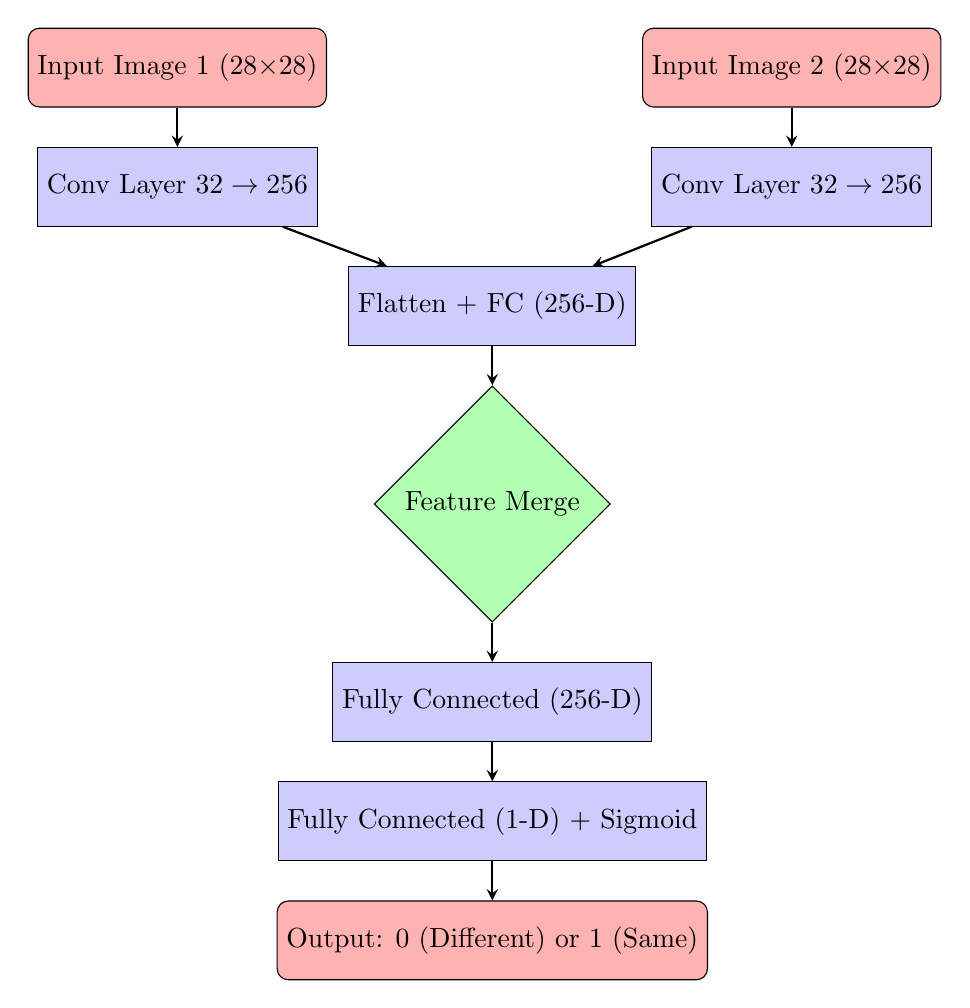
\begin{tikzpicture}[node distance=0.5cm]
  
        % Input Layer
        \node (input1) [startstop] {Input Image 1 (28$\times$28)};
        \node (input2) [startstop, right=of input1, xshift=3.5cm] {Input Image 2 (28$\times$28)};
  
        % Convolutional Layers
        \node (conv1) [process, below=of input1] {Conv Layer $32 \rightarrow 256$};
        \node (conv2) [process, below=of input2] {Conv Layer $32 \rightarrow 256$};
  
        % Fully Connected Layer (Shared)
        \node (fc1) [process, below=of conv1, xshift=4cm] {Flatten + FC (256-D)};
  
        % Feature Merging
        \node (merge) [decision, below=of fc1] {Feature Merge};
  
        % Classifier
        \node (fc2) [process, below=of merge] {Fully Connected (256-D)};
        \node (fc3) [process, below=of fc2] {Fully Connected (1-D) + Sigmoid};
  
        % Output
        \node (output) [startstop, below=of fc3] {Output: 0 (Different) or 1 (Same)};
  
        % Arrows
        \draw [arrow] (input1) -- (conv1);
        \draw [arrow] (input2) -- (conv2);
  
        
        \draw [arrow] (conv1) -- (fc1);
        \draw [arrow] (conv2) -- (fc1);
  
        \draw [arrow] (fc1) -- (merge);
        \draw [arrow] (merge) -- (fc2);
        \draw [arrow] (fc2) -- (fc3);
        \draw [arrow] (fc3) -- (output);
  
    \end{tikzpicture}
  \end{center}
  \caption{Siamese CNN Architecture}
  \label{fig:siamese_cnn}
  \end{figure}
  
\newpage
\section*{Problem 4}
\subsection*{Introduction}
For this experiment, we compare the performance of three popular optimizers: Stochastic Gradient Descent (SGD), SGD with momentum, and ADAM on the CIFAR-10 dataset using a ResNet. We investigate how the choice of learning rate affects the optimizers' convergence speed and final performance. The goal is to identify the optimal learning rate for each optimizer that yields the best classification accuracy on the CIFAR-10 test set.

\subsection*{Experimental Setup}
We train a ResNet on the CIFAR-10 dataset using three optimizers: plain SGD, momentum SGD (momentum = 0.9), and Adam. To keep the experiment consistent, we use the same ResNet architecture, training hyperparameters, and data preprocessing for all optimizers. The learning rate is varied for each optimizer, with values of 0.01, 0.02, and 0.05 tested. The model is trained on the CIFAR-10 training set and evaluated on the test set.

We train the each model for 10000 iterations with a batch size of 128 and a weight decay of 0.0001. The model is evaluated on the full CIFAR-10 test after each epoch, and the test loss and accuracy are recorded. The training time is also measured to assess the optimizers' efficiency.

\subsection*{Results and Discussion}

The train, test loss, and accuracy curves for each optimizer and learning rate are plotted in Figure \ref{fig:exp_results}. Key metrics are summarized in Table \ref{tab:exp_results}.

\begin{figure}[ht]
  \centering
  % Add subfigures
  \begin{subfigure}{0.45\textwidth}
    \includegraphics[width=\textwidth]{images/q4_train_loss.png}
    \caption{Training Loss}
  \end{subfigure}
  \hspace{0.5cm}
  \begin{subfigure}{0.45\textwidth}
    \includegraphics[width=\textwidth]{images/q4_test_loss.png}
    \caption{Test Loss}
  \end{subfigure}
  
  \begin{subfigure}{0.45\textwidth}
    \includegraphics[width=\textwidth]{images/q4_test_acc.png}
    \caption{Test Accuracy}
  \end{subfigure}
  \caption{Experimental Results for Different Optimizers and Learning Rates}
  \label{fig:exp_results}
\end{figure}

We also plot the confusion matrices for each optimizer and learning rate in Figure \ref{fig:conf_matrices}. The confusion matrices provide insights into the model's classification performance for each optimizer and learning rate. 

\begin{figure}
  \centering
  \includegraphics[width=0.6\textwidth]{images/q4_conf_matrices.png}
  \caption{Confusion Matrices for Different Optimizers and Learning Rates}
  \label{fig:conf_matrices}
\end{figure}


\begin{table}[ht]
  \centering
  \begin{tabular}{|l|l|l|l|l|l|l|l|}
    \hline
    \textbf{Optimizer} & \textbf{LR} & \textbf{Test Loss} & \textbf{Acc (\%)} & \textbf{Precision} & \textbf{Recall} & \textbf{F1} & \textbf{Time (sec)} \\
    \hline
    Adam & 0.01 & 0.6479 & 77.67 & 0.7784 & 0.7767 & 0.7748 & 1429.49 \\
    Adam & 0.02 & 0.8910 & 68.05 & 0.7125 & 0.6805 & 0.6761 & 1450.36 \\
    Adam & 0.05 & 1.2755 & 53.53 & 0.5329 & 0.5353 & 0.5246 & 1456.67 \\
    \hline
    Momentum SGD & 0.01 & 0.5214 & 83.24 & 0.8470 & 0.8324 & 0.8349 & 1427.31 \\
    Momentum SGD & 0.02 & 0.4649 & 84.71 & 0.8508 & 0.8471 & 0.8465 & 1442.08 \\
    Momentum SGD & 0.05 & 0.4931 & 83.91 & 0.8454 & 0.8391 & 0.8350 & 1477.96 \\
    \hline
    SGD & 0.01 & 0.7929 & 72.16 & 0.7221 & 0.7216 & 0.7190 & 1432.62 \\
    SGD & 0.02 & 0.7463 & 74.74 & 0.7529 & 0.7474 & 0.7454 & 1427.47 \\
    SGD & 0.05 & 0.0000 & 10.00 & 0.9100 & 0.1000 & 0.0182 & 1428.63 \\
    \hline
  \end{tabular}
  \caption{Experimental Results for Different Optimizers and Learning Rates}
  \label{tab:exp_results}
\end{table}  

Based on the results, we can conclude that the choice of optimizer and learning rate significantly impacts the model's performance. Momentum SGD with a learning rate of 0.02 achieves the best test accuracy of 84.71\% and the lowest test loss of 0.4649. This optimizer also exhibits the highest precision, recall, and F1 score among all configurations. Adam performs well with a learning rate of 0.01, achieving a test accuracy of 77.67\%. However, it shows a significant drop in performance with higher learning rates. Plain SGD is the least effective optimizer, with a test accuracy of 74.74\% at a learning rate of 0.02. The model trained with SGD and a learning rate of 0.05 fails to converge, resulting in a test accuracy of 10.00\%. 



\newpage
\section*{Appendix}
\subsection*{Code for Problem 1}
Attached and available at the following link: \url{https://www.kaggle.com/code/hurryingauto3/aml-hw2-q1}.

\subsection*{Code for Problem 2}
Attached and available at the following link: \url{https://www.kaggle.com/code/hurryingauto3/aml-hw2-q2}.

\subsection*{Code for Problem 3}
Attached and available at the following link: \url{https://www.kaggle.com/code/hurryingauto3/aml-hw2-q3}.

\subsection*{Code for Problem 4}
Attached and available at the following link: \url{https://www.kaggle.com/code/hurryingauto3/aml-hw2-q4}.

\includepdf[pages=-]{aml-hw2-q1.pdf}
\includepdf[pages=-]{aml-hw2-q2.pdf}
\includepdf[pages=-]{aml-hw2-q3.pdf}
\includepdf[pages=-]{aml-hw2-q4.pdf}


\end{document}
